\chapter{Introduction}

A big field in astronomy and particle physics ever since Victor Hess discovered
the extraterrestrial origin of the atmospheric ionization
is astroparticle physics. Despite falling out of favor for a few years
when terrestrial particle accelerators reached ever higher energies,
the field is very famous today. One of the reasons being that
even the biggest accelerators, like the LHC, got to a point where
increasing collision energies gets ever more difficult.

Despite all the effort and numerous achievements,
in the field of astroparticle physics
there are still many questions left.
Some of the prominent ones are:
\begin{itemize}
    \item{How does general relativity work at in extreme cases and 
	what happens at the singularities?}
    \item{Which particles form the dark matter?}
    \item{Why is the universe expanding and what is dark energy?}
    \item{How do cosmic rays get accelerated to the highest energies?}
    \item{Are neutrinos majorana particles?}
\end{itemize}

Nowadays there exists a wide range of experiments trying to
solve these questions. They focus on different particles and detection
mechanisms to detect
extraterrestrial particle sources, which is why
the term multi messenger astronomy is widely used.


\section{The origins of astroparticle physics}
1785 Charles-Augustin de Coulomb first described the electrostatic forces 
and found out that the electric charge on an electroscope can
reduce over time although no contact has been made \cite{???}

Much later, in 1879, William Crookes noted that the speed of the discharge
depended on the pressure of the surrounding air 
\cite{doi:10.1098/rstl.1879.0076}.
This lead to the insight that the air must be ionized, but an 
explanation was not yet available.

A step towards the solution of this mistery was the discovery 
of radioactivity by Henri Becquerel in 1896 
\cite{becquerel1896emission} and the following studies 
of Marie and Pierre Curie \cite{????}, 
that awarded all three of them the nobel prize \cite{???}

Around 1900 (Genauer?):
With experimental improvements, led by Charles Thomson Rees Wilson,
Julius Elster and Hans Friedrich Geitel, quantitative measurements 
of the spontaneous discharge became possible \cite{\\multiple??}.
For this the electroscope was insulated into a closed vessel.
With these measurements it became evident that the source 
of the ionised particles was indeed outside of the vessel.
The obvious explanation seemed to be, that the surrounding material 
emitted radioactivity \cite{bookap}.
Also Wilson proposed a penetrating extraterrestrial radiation, 
he could not support his theory with experimental results, 
so the idea was dropped \cite{????im zweifel bookap}.

By 1909, SOMEONE found, that the mysterious radiation was also 
penetrating metal, which only left $\gamma$-radiation as 
possible source. Besides radioactivity in the earth crust or atmosphere,
another possible source was assumed to be the sun \cite{bookap}.

To test these hypotheses, the following years included many experiments 
above or under sea level to measure if the radiation strength changes.

In 1909 Theodor Wulff measured the radiation on top of the 
eiffel tower in paris. 
\cite{wulf1909atmosphare} -> finden und lesen!
Assuming that most radiation came from the 
earth crust, the decrease was less than expected.

Balloon flights of Albert Gockel in 1909 
\cite{gockel1909atmosphare} -> finden und lesen, ggf englische version?
and underwater experiments of Domenico Pacini in 1910 
lead to the conclusion that most of the radiation must indeed be
of extraterrestrial origin.

- pacini, 1910, underwater: a lot must be not from earth
\cite{2011arXiv1101.3015P}
- gockel, 1909: balloon -> same interpretation, still doubts in the community



- hess, 1911-1921: 7 ballons 
-> increase at some height 
-> not from earth and probaly extraterrestrial because same at night
\cite{Hess:1912srp}
- kollhörster, 1929 : confirmation
\cite{bothe1929wesen}
-> hess: "höhenstrahlung"  \cite{myssowsky1926versuche},
milikan: cosmic rays \cite{millikan1928origin}

- clay, 1927: dependent from magnetic field -> charged particles
\cite{clay1927penetrating}
- alvarez+compton/rossi/johnson -> more form west than east -> positive charge
\cite{PhysRev.43.835}
\cite{Rossi1933}
\cite{PhysRev.43.834}

- anderson 1933: cosmic rays in cloud chamber -> antimatter discovery
\cite{PhysRev.43.491}
-rossi 1934/auger, 1937: coincident event in geiger müller at large distances -> particle showers -> high energy primary interacts in atmosphere
\cite{PhysRev.45.212}
\cite{RevModPhys.11.288} (paper ist von 39, der hat halt so lange gebraucht)

- more particles got found -> pions, muons
cite paper der entdeckungen -> ws4
- cern, 1954 -> do we even need astro anymore? fermi: we can get up to 5000TeV in theory -> lulz
-

- turns out its still useful, despite falling out of favor for some while
- today we observe on four channels -> multimessenger astronomy with growing collaboration
- neutrinos fehlen hier noch komplett! -> entdeckung als vorletzten punkt hier
- gravitationswellenentdeckung als letzten punkt hier

\section{Modern Multimessenger astronomy}

The sources of extraterrestrial radiation can be ...
(Vorgänge kurz anreißen, agns, supernovae...)
und key areas of research. func-ray scheint da einen guten Überblick zu haben. bookap auch, aer sehr lang
hier auch kurz wofür man speziell IACTs nutzt

Nowadays we observe these processes by looking at one of four channels: 
\begin{enumerate}
	\item Electromagnetic radiation
	\item (Charged) cosmic rays
	\item $\nu$-radiation
	\item Gravitational waves
\end{enumerate}

All of these have vastly different properties and require different experiments.
In the recent years, it became a common thing to observe the same sources 
on different channels to learn more about the processes that happen at 
these far distant sources. This is what is often times 
referred to as multi messenger astronomy (cite some mma paper, eg magic looking at an icecube alert).

Before we focus on the special field of imaging air cherenkov telecopes, we will have
a brief look at the different channels.

- bild von der astrovorlesung einfügen und erklären!
\begin{figure}
	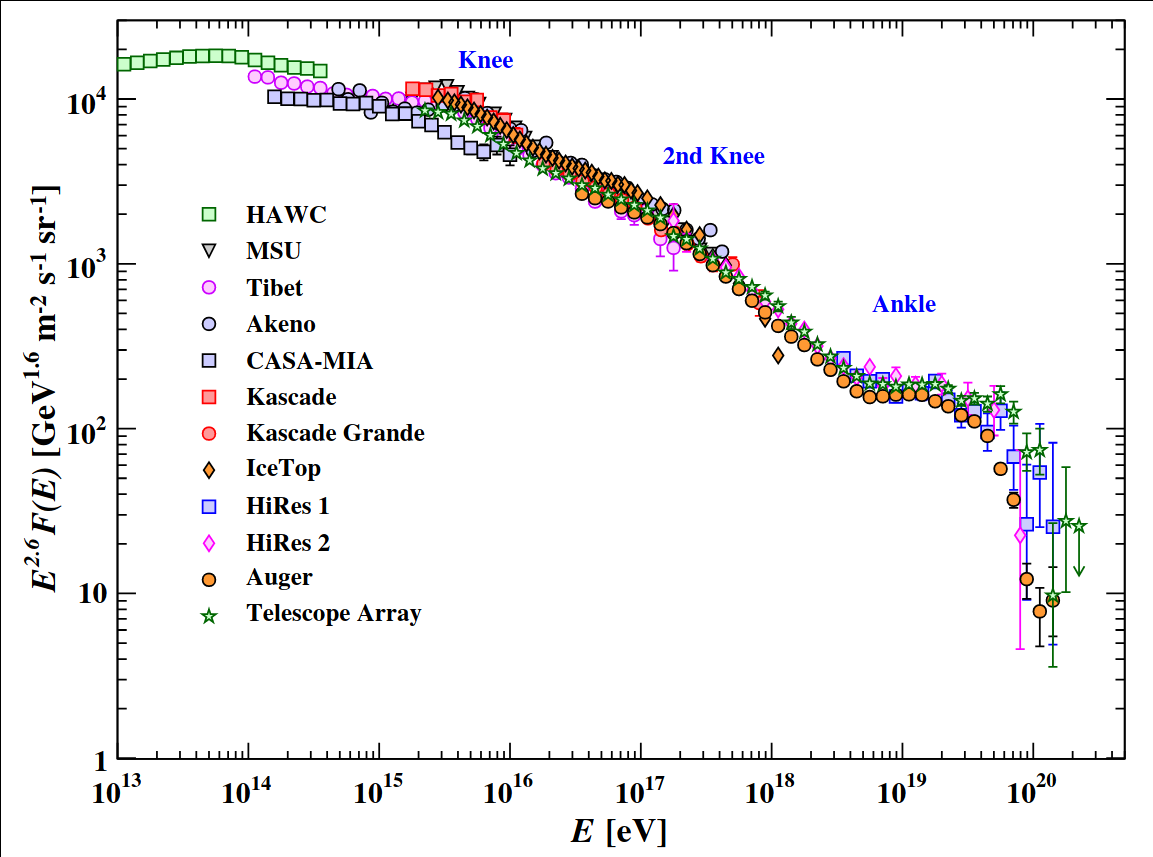
\includegraphics[width=.8\textwidth]{images/cr_spectrum.png}
	\label{fig:multi_messenger}
	\caption{Visualisation of the behaviours of different astronomy messengers. Photons and neutrinos 
		travel the universe without deflection. Charged cosmic rays get deflected by interstellar
		magnetic fields and thus do not allow for a assignment to a cosmological source.
		Neutrinos interact way less than photons both in the universe and in the detector 
		which requires the detectors to be of huge areas. Gravitational waves anyone?
	}
\end{figure}


\subsection{Charged cosmic rays}
The term charged cosmic rays summates all types of charged particles from
extra terrestrial sources with the main proportion seemingly being protons
\cite{something something}


Cosmic rays can similarly be observed both directly and indirectly (werte falsch, anpassen).
- kurze erklärung davon


Figure \ref{fig:cr_spectrum} shows the flux of charged cosmic rays over 
many orders of magnitude in energy which mainly follows 
a power law $E^{-\gamma}$ with gamma somewhere between 
2.7 and 3.3. Deviations from this crude approximation are 
usually referred to as the first and second knee and the ankle 
at $5 10^{15}, 2 10^{17} and 5 10^{18}$ eV respectively.

\begin{figure}
	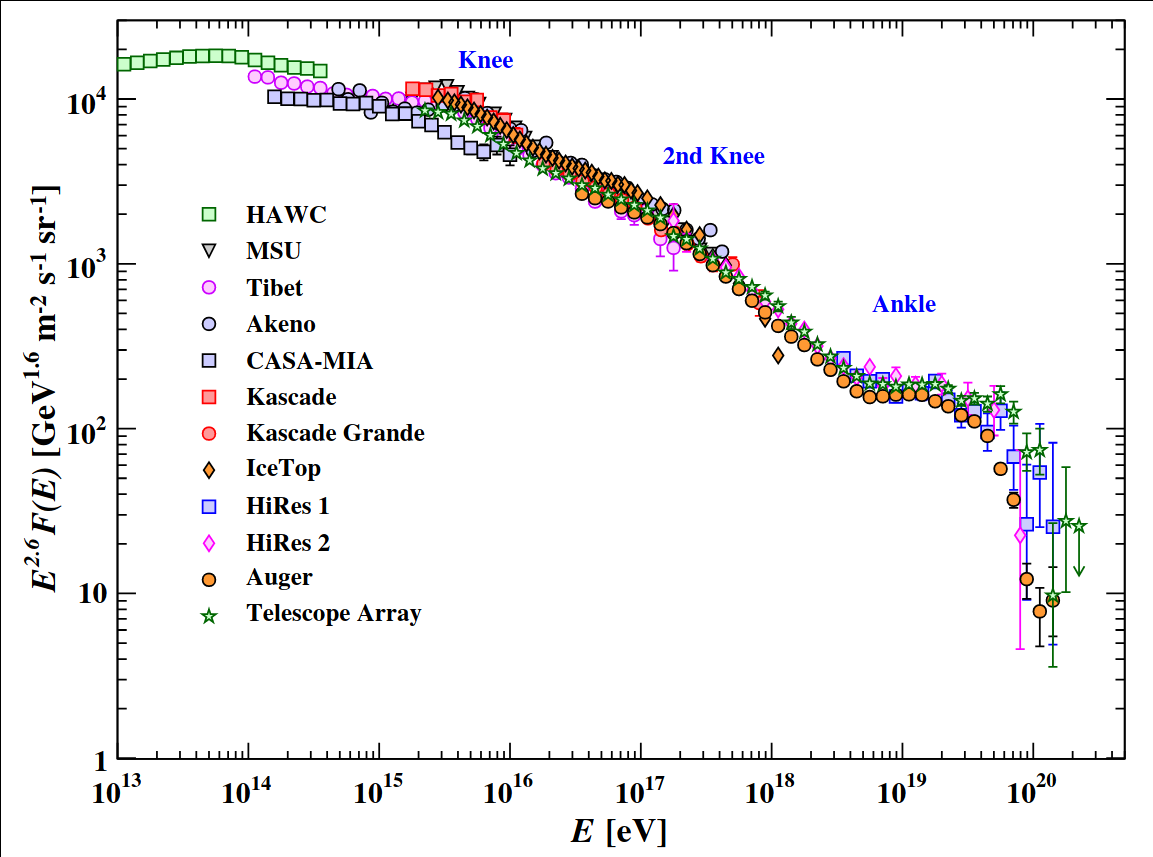
\includegraphics[width=.8\textwidth]{images/cr_spectrum.png}
	\label{fig:cr_spectrum}
	\caption{Combined plot of the cosmic ray spectrum, measured by different air shower experiments. \cite{pdg2019}. 
		The original data were taken from reports from \cite{Alfaro:2017cwx}, 
		\cite{1991ICRC....2...85F}, more here. or leave it altogether.
	}
\end{figure}


At the very highest energies, the flux seems to rapidly decrease, which may point towards a maximum energy
tat cosmological sources can produce or towards destructive interaction with 
the cosmic microwave background \cite{bookap}.

\subsection{Electromagnetic radiation}
In contrast to charged cosmic rays, $\gamma$-particles point towards
their sources, allowing to search for sources of radiation.
In astronomy electromagnetic radiation refers to $\gamma$-particles at all wavelength,
the term $\gamma$-radiation being assigned to the very highest energy particles.
The energy span is usually divided into different ranges, as can be seen in \ref{fig:em_spectrum}

\begin{figure}
	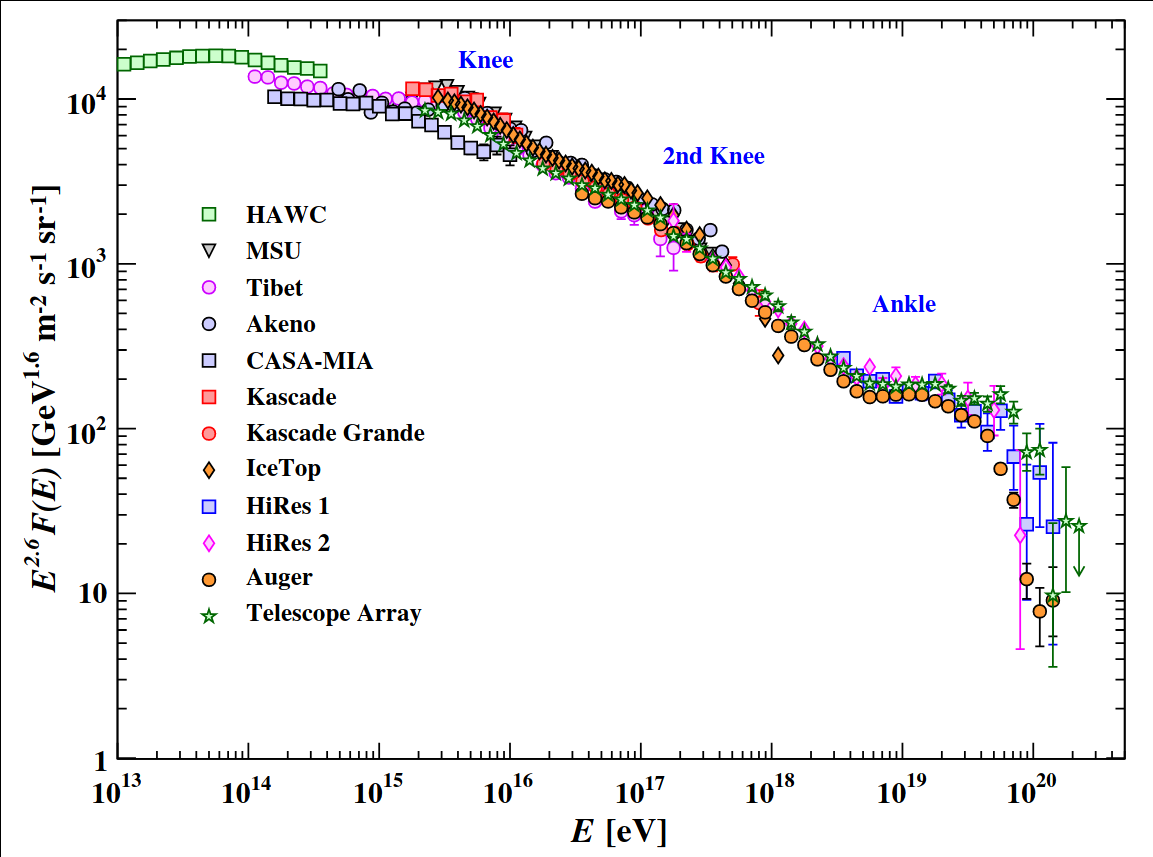
\includegraphics[width=.8\textwidth]{images/cr_spectrum.png}
	\caption{Search for another pic in a paper and cite properly}
	\label{fig:em_spectrum}
\end{figure}


Emitted photons can be observed either directly
from outside the atmosphere via satellites or indirectly
via ground based gamma astronomy. In the later case
IACT's are used to detect electromagnetic showers induced
by the collision of high energy photons with partticles in the atmosphere.
An example for direct observation could be the Fermi satellite (citation needed),
an example for ground based observation could be the
MAGIC-experiment (citation needed).

- smth bout the spectrum with image, bookap has smth but we might find a better one.

\subsection{Neutrinos}
Even less affected by interations on the way from the source to the earth are neutrinos.
Due to their small interaction cross sections and no electric charge, they 
suffer very little from absorption or deflection.
For very much the same reasons detecting neutrinos is much harder
than detecting photons or charged particles.

The small cross section requires to build huge detectors, 
the ICECUBE having a detector volume of \SI{1}{\kilo\meter^3}(cite that).

because of
their small cross-sections. This leads to thousands (größenordnung checken) of
neutrinos passing us continiusly without us even noticing.
For this reason neutrino detectors need to be very large. One example
of such a detector is the ICECUBE detector in ??? (ctation needed).

\subsection{Gravitational waves}
Gravitational waves are the newest channel available for observation.
We can detect them using large size interferometers such as
the LiGO's three detectors (citation needed).



Ground-based cherenkov astronomy focuses on either $\gamma$-rays or cosmic rays


\section{Detection of gamma-rays with ground based telescopes}
The primary particles of gamma or cosmic rays cannot be 
observed with IACTs directly. Instead one can measure the secondary particles
that emerge from the particles interaction with matter.

If the primary energy is high enough, the resulting 
particles can interact with the atmosphere themself, thus starting a 
cascade of secondary particles.

Depending on whether the primary particle is 
a photon/electron/positron or a heavier particle such as a proton 
or iron core, the interactions vary.

This leads to the separation of electromagnetic and hadronic showers.
If the experiment is primarly looking for 
gamma rays, e.g. if measuring a known source like the Crab Nebula, 
the hadronic showers can be treated as background.
As hadronic showers get observed much more frequently, 
the identification of the primary particle type is a very important 
task, often times referred to as gamma-/hadron-separation.

To understand how these showers differ, we will have a very brief look
at the relevant interactions (at primary particle energies in the 
region of modern IACTs).
!!Energiebereiche besser einschränken!!!


\subsection{Electromagnetic showers}
Electromagnetic showers consist mainly of three types of particles:
\begin{enumerate}
	\item{Photons $\gamma$}
	\item{Electrons $e^-$}
	\item{Positrons $e^+$}
\end{enumerate}

The main interaction for high energy photons is pair 
production, generating an $e^+-/e^--$pair where the energy of 
the secondary particles equals the photon energy.
On the other hand high energy electrons (and positrons) lose 
most of their energy by radiation, leading to a photon with 
an energy close to the electron energy.

Only at lower particle energies other interaction forms show their impact,
with particle scattering and ionisation 
leading to more continous energy losses.

Although the energy losses are mainly negligible, 
the most important interaction for the detection with IACTs is 
cherenkov radiation: High energy charged particles pass through 
matter faster than the speed of light in the medium. This leads
to the emittance of near-visible photons that get detected 
in the telescopes camera. 

These assumptions lead to the most basic model of an 
electromagnetic shower, proposed by Bhabha and Heitler in 1937
\cite{doi:10.1098/rspa.1937.0082}.
Today monte carlo calculations get used to simulate the properties 
of particle showers in the atmosphere.
The most common software in the field of IACTs is referred to as
CORSIKA \cite{Engel:2018akg}.

\subsection{Hadronic showers}
Hadronic showers include all the interactions known from 
electromagnetic showers, but adds nuclear interactions on top.
These lead to non-negligible additional energy losses 
and the creation of secondary hadronic particles.


Approximations are more difficult to do and simulations 
become the only way to reasonably calculate shower behaviour.

At the end of the shower most particles have decayed into the 
lightest hadronic particles, pions ($\pi^0, \pi^+, \pi^-$), of which the neutral pions 
rapidly decay into photons.
\cite{bookap} (vlt gibts da bessere quellen) states that on average
roughly a third of the pions are neutral pions. This means that 
a third of the hadronic shower eventually becomes a electromagnetic 
(sub-)shower.


\subsection{Measuring events}
As stated earlier, IACTs measure particle showers by their emittance of cherenkov 
light. This light gets collected by a large mirror (or a composition of 
multiple smaller mirrors) and projected onto a camera system mounted some 
meters above the mirror. 
With this setup IACTs usually reach a field of view of 
a few degree (magic: wert, zitat, hess: wert, zitat, veritas: wert, zitat)
Figure \ref{fig:iact_mirror_camera} illustrates this 
setup.

Upon detection of a shower, the usual tasks include reconstructing 
three key properties of the primary particle:
\begin{enumerate}
	\item{Particle type (mostly photon or hadronic)}
	\item{Energy}
	\item{Direction (leading to the source position)}
\end{enumerate}

The base idea resolves around describing the 
shower image as ellipse and calculating the hillas parameters \cite{hillas params paper}.
This allows to describe the shower image with only a handful of parameters.


Usually the reconstruction can be improved heavily by cleaning the image first.
Figure \ref{fig:shower_cleaning} shows a simulated $\gamma$-induced shower 
in the camera of the Large Sized Telescope (see section \ref{sec:lst} for more details)
before and after cleaning


\begin{figure}
	\centering
	\begin{subfigure}{.5\textwidth}
  		\centering
  		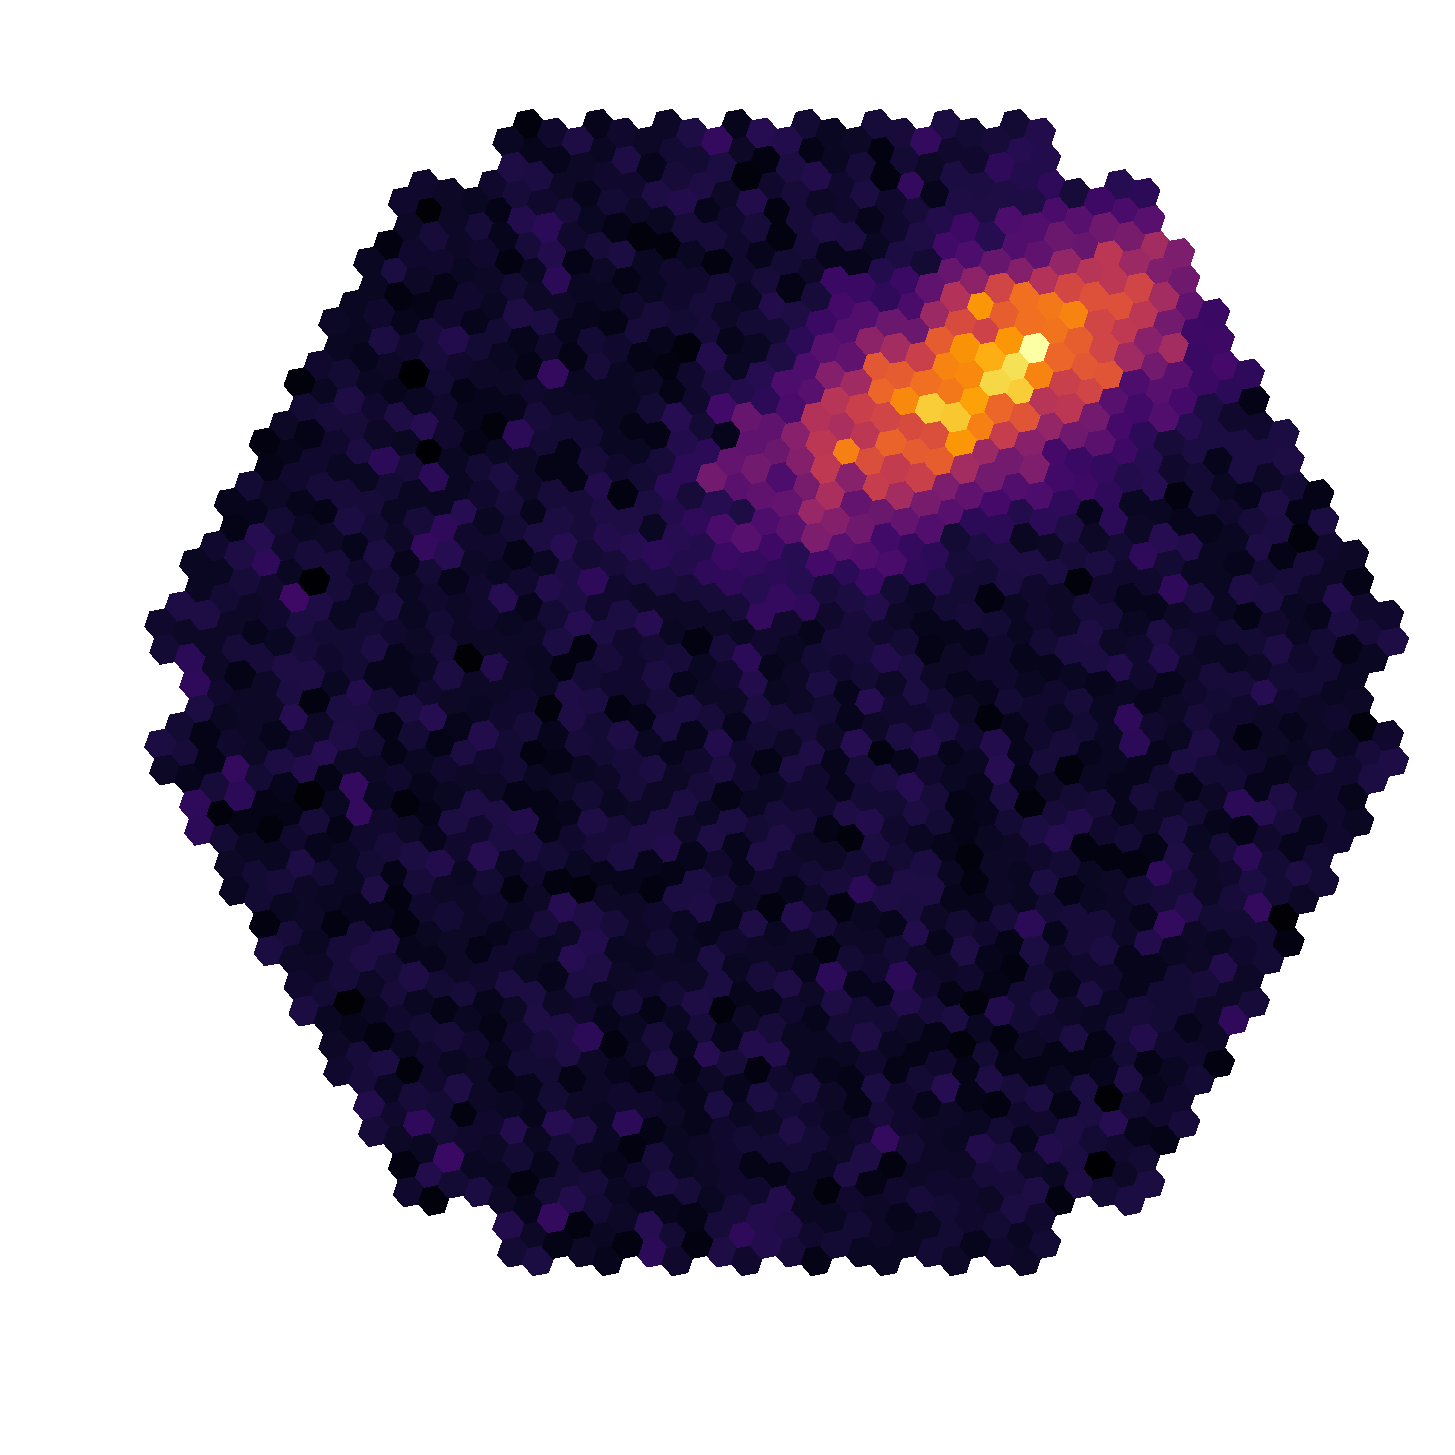
\includegraphics[width=.9\linewidth]{Plots/hillas_raw.pdf}
		\caption{raw image}
	\end{subfigure}%
	\begin{subfigure}{.5\textwidth}
 		\centering
		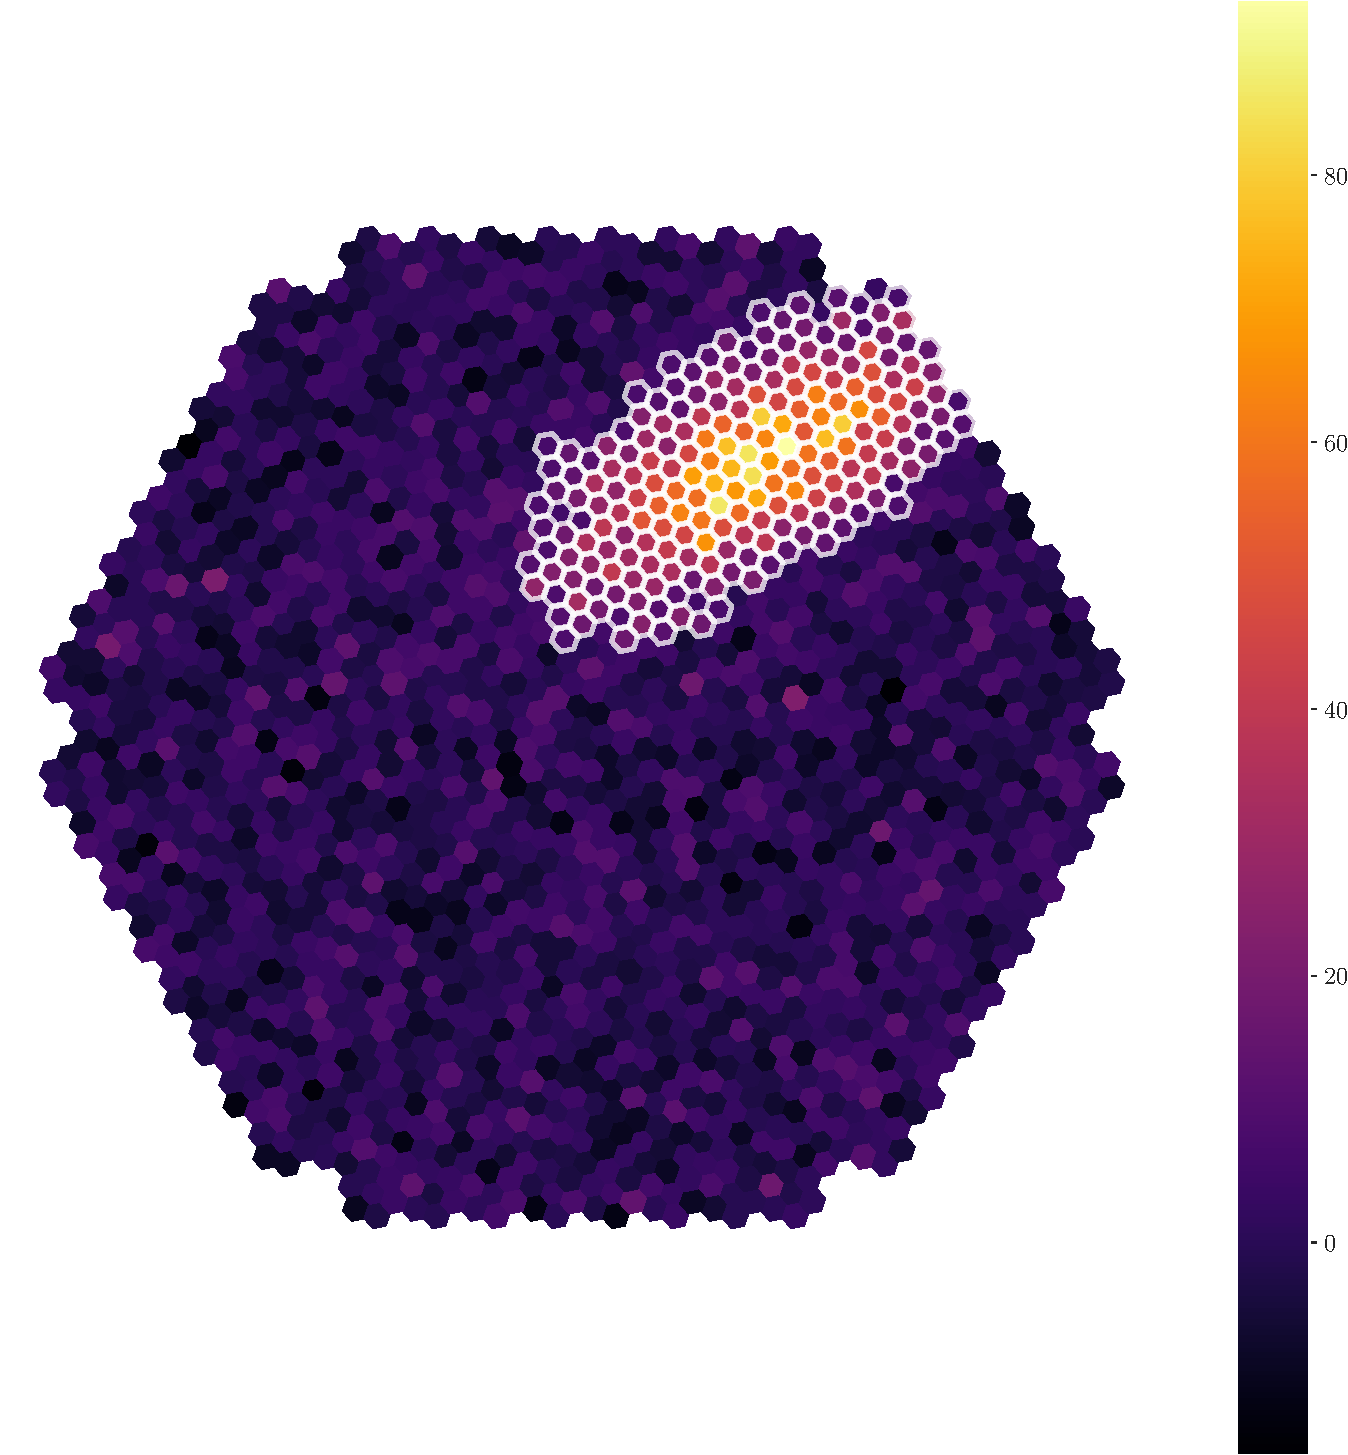
\includegraphics[width=.9\linewidth]{Plots/hillas_cleaned.pdf}
 		\caption{cleaned image}
	\end{subfigure}
	\caption{A figure with two subfigures}
	\label{fig:shower_cleaning}
\end{figure}

From the reconstructed image, the hillas parameters can be calculated.
An illustration with the hillas-ellipse on top of the camera image 
for the same image can be seen in figure \ref{fig:hillas_params}.

\begin{figure}
	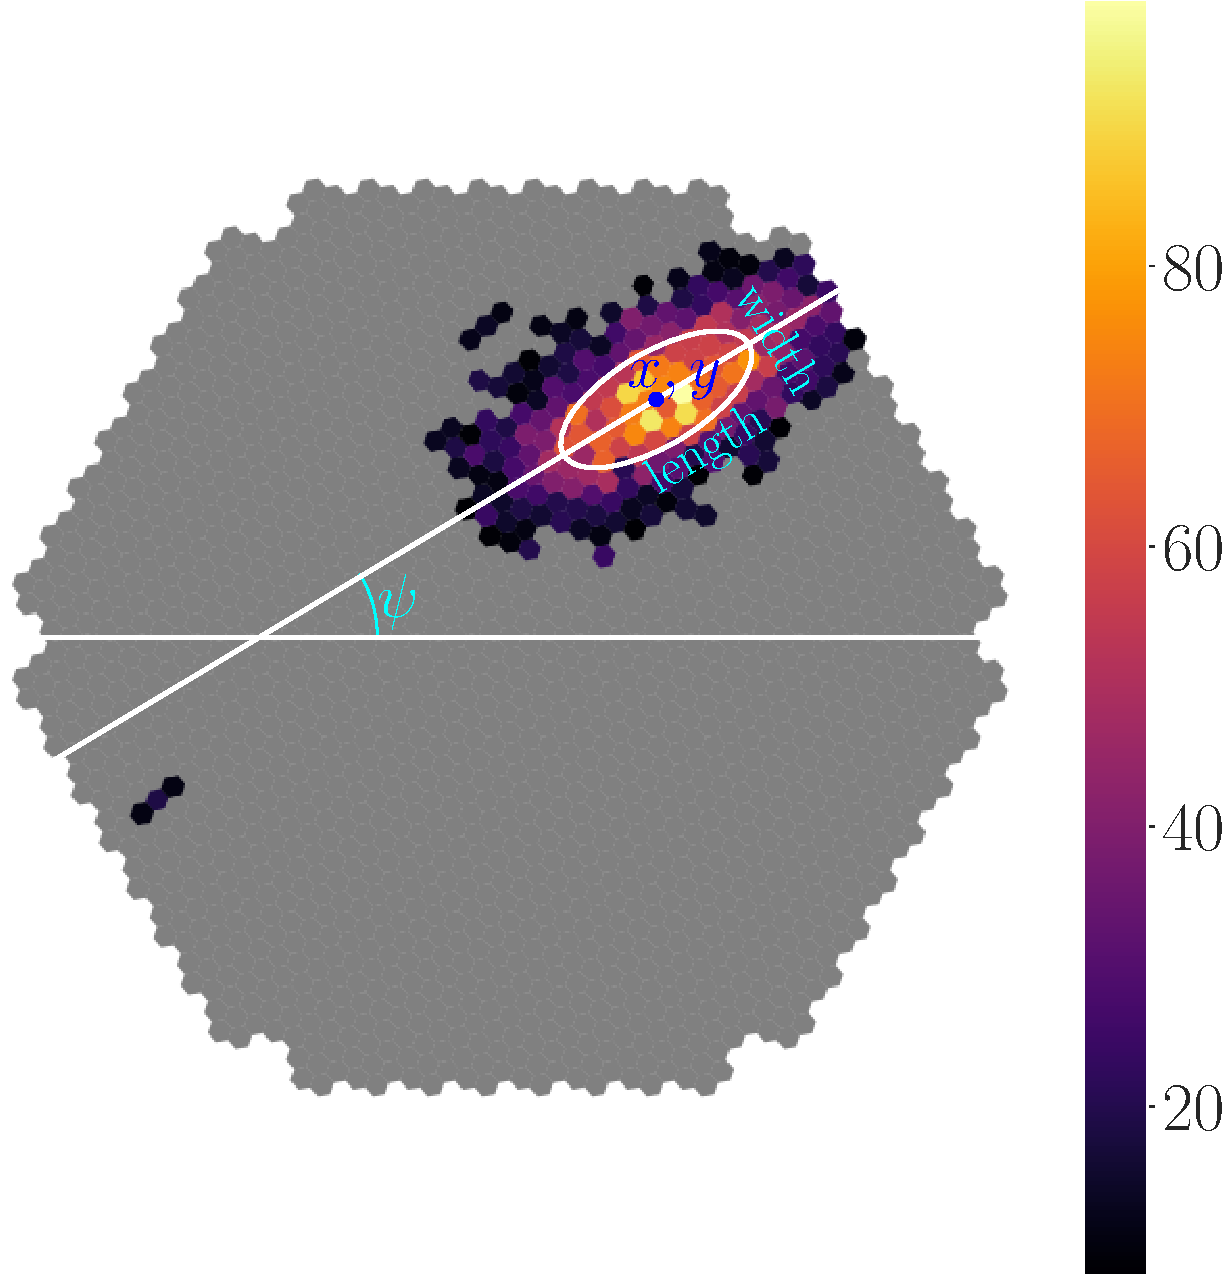
\includegraphics[width=.8\textwidth]{Plots/hillas_cleaned_params.pdf}
	\caption{hillas params}
	\label{fig:hillas_params}
\end{figure}

With the hillas parameters calculated, the reconstruction of the 
primary particles properties can be done.

In first order one can predict the shower origin by 
transforming the center of gravity(cog) of the image onto the sky plane.
More sophisticated methods assume that the 
center of gravity is displaced relative to the
real source position depending on the angle the photon arrived at the telescope.
This angle also leads to more eccentric ellipses the higher the angle is.
If one assumes the true source position to be on the main shower axis of the ellipse,
finding this position simplifies to finding a point on the main shower axis.
This is often times referred to as DISP-method, first used at magic? \cite{someting magic idk}
Monoscopic experiments also need to resolve the head-tail-ambiguity:
Knowing the distance from the cog leaves two possible points, one on either side 
of the ellipse, as can be seen in !!!!Bild erstellen!!!!

Stereoscopic experiments can resolve this ambiguity by combining the images from 
multiple telescopes.


The primary energy is mostly described by the contained light in the image combined with 
an estimate of how much of the light missed the camera. 


The particle type can be reconstructed 
by looking at the image shape.
A representation of different shower types can be seen in \ref{fig:compare_showers}

\begin{figure}
	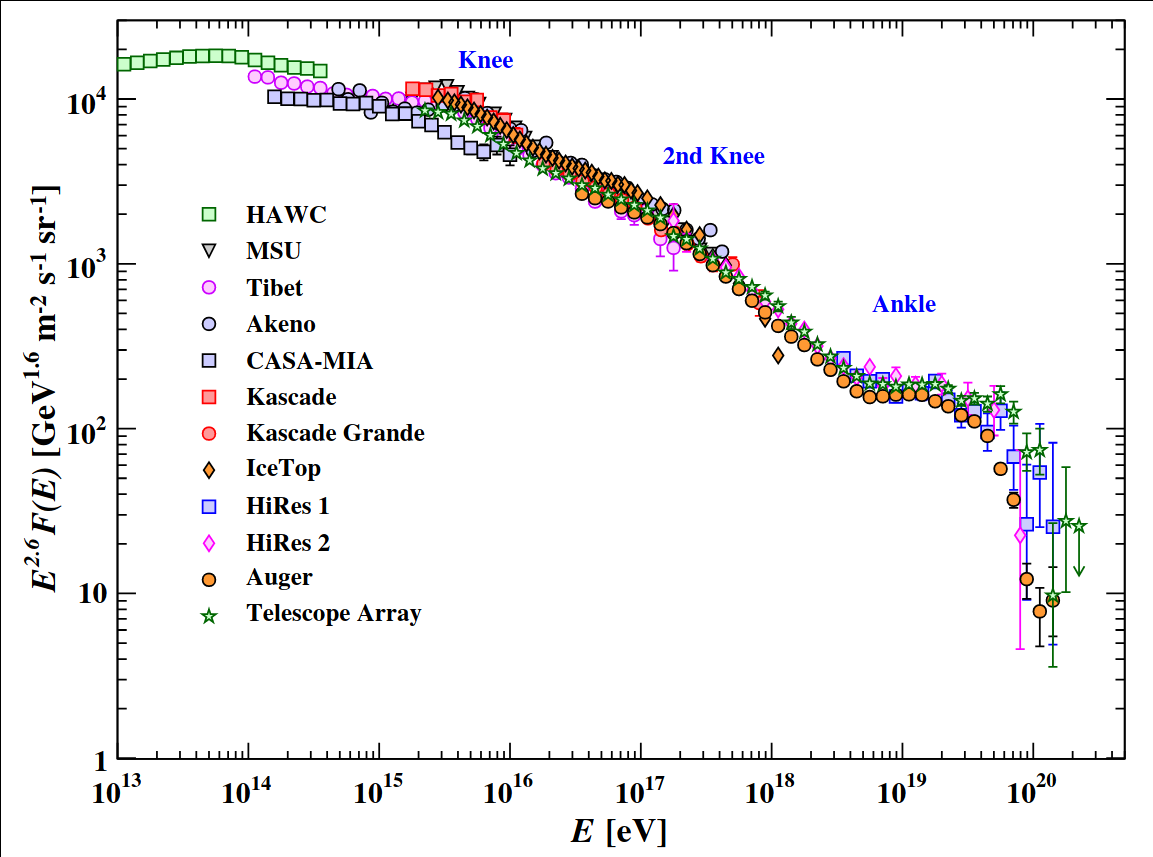
\includegraphics[width=.8\textwidth]{images/cr_spectrum.png}
	\caption{compare diff types, explain diffs  and cite source}
	\label{fig:compare_showers}
\end{figure}

Gamma-showers are usually more compact and better described via an ellipse.








!!!!!!!!!!!!!photon/gamma/$\gamma$ showers konsistent machen, gamma showers erklären!!!!!!!!!!

